\Chapter{Processz ütemezés}

\Section{Az ütemezési probléma}

\Section{Elterjedt ütemezési stratégiák}

\SubSection{$\mathcal{O}(1)$}

\SubSection{$\mathcal{O}(n)$}

\SubSection{Completely Fair Scheduler}

\begin{table}[h]
\centering
\caption{A processz végrehajtásához szükséges idő}
\label{tab:processtimes}
\begin{tabular}{|c|c|}
\hline
Processz & idő \\
\hline
A & 8ms \\
B & 4ms \\
C & 16ms \\
D & 4ms \\
\hline
\end{tabular}
\end{table}

\begin{table}[h]
\centering
\caption{A processzekre jutó időszeletek}
\label{tab:timeslices}
\begin{tabular}{|c|c|c|c|c|c|c|c|c|}
\hline
A & 1 & 2 & 3 & 4 & 6 & 8 & & \\
B & 1 & 2 & 3 & 4 & & & & \\
C & 1 & 2 & 3 & 4 & 6 & 8 & 12 & 16 \\
D & 1 & 2 & 3 & 4 & & & & \\
\hline
\end{tabular}
\end{table}

\begin{figure}[h]
\centering
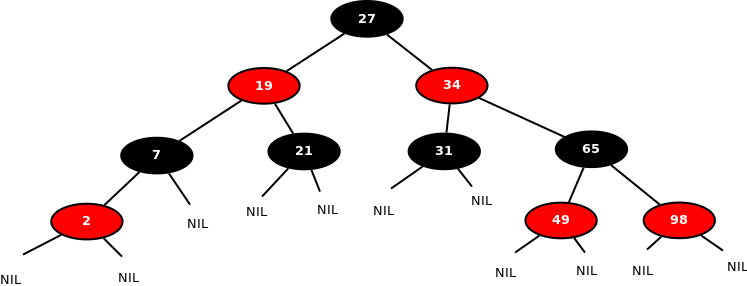
\includegraphics[width=\textwidth]{images/rb_tree.png}
\caption{Piros fekete fa a processz prioritás értékekkel}
\label{fig:rb_tree}
\end{figure}
